 \thispagestyle{gocconone}
\pagestyle{gocco}
\everymath{\color{gocco}}
\graphicspath{{../gocco/pic/}}
\blfootnote{$^1${\color[named]{gocco}Tp. Hồ Chí Minh.}}
\begingroup
\AddToShipoutPicture*{\put(0,616){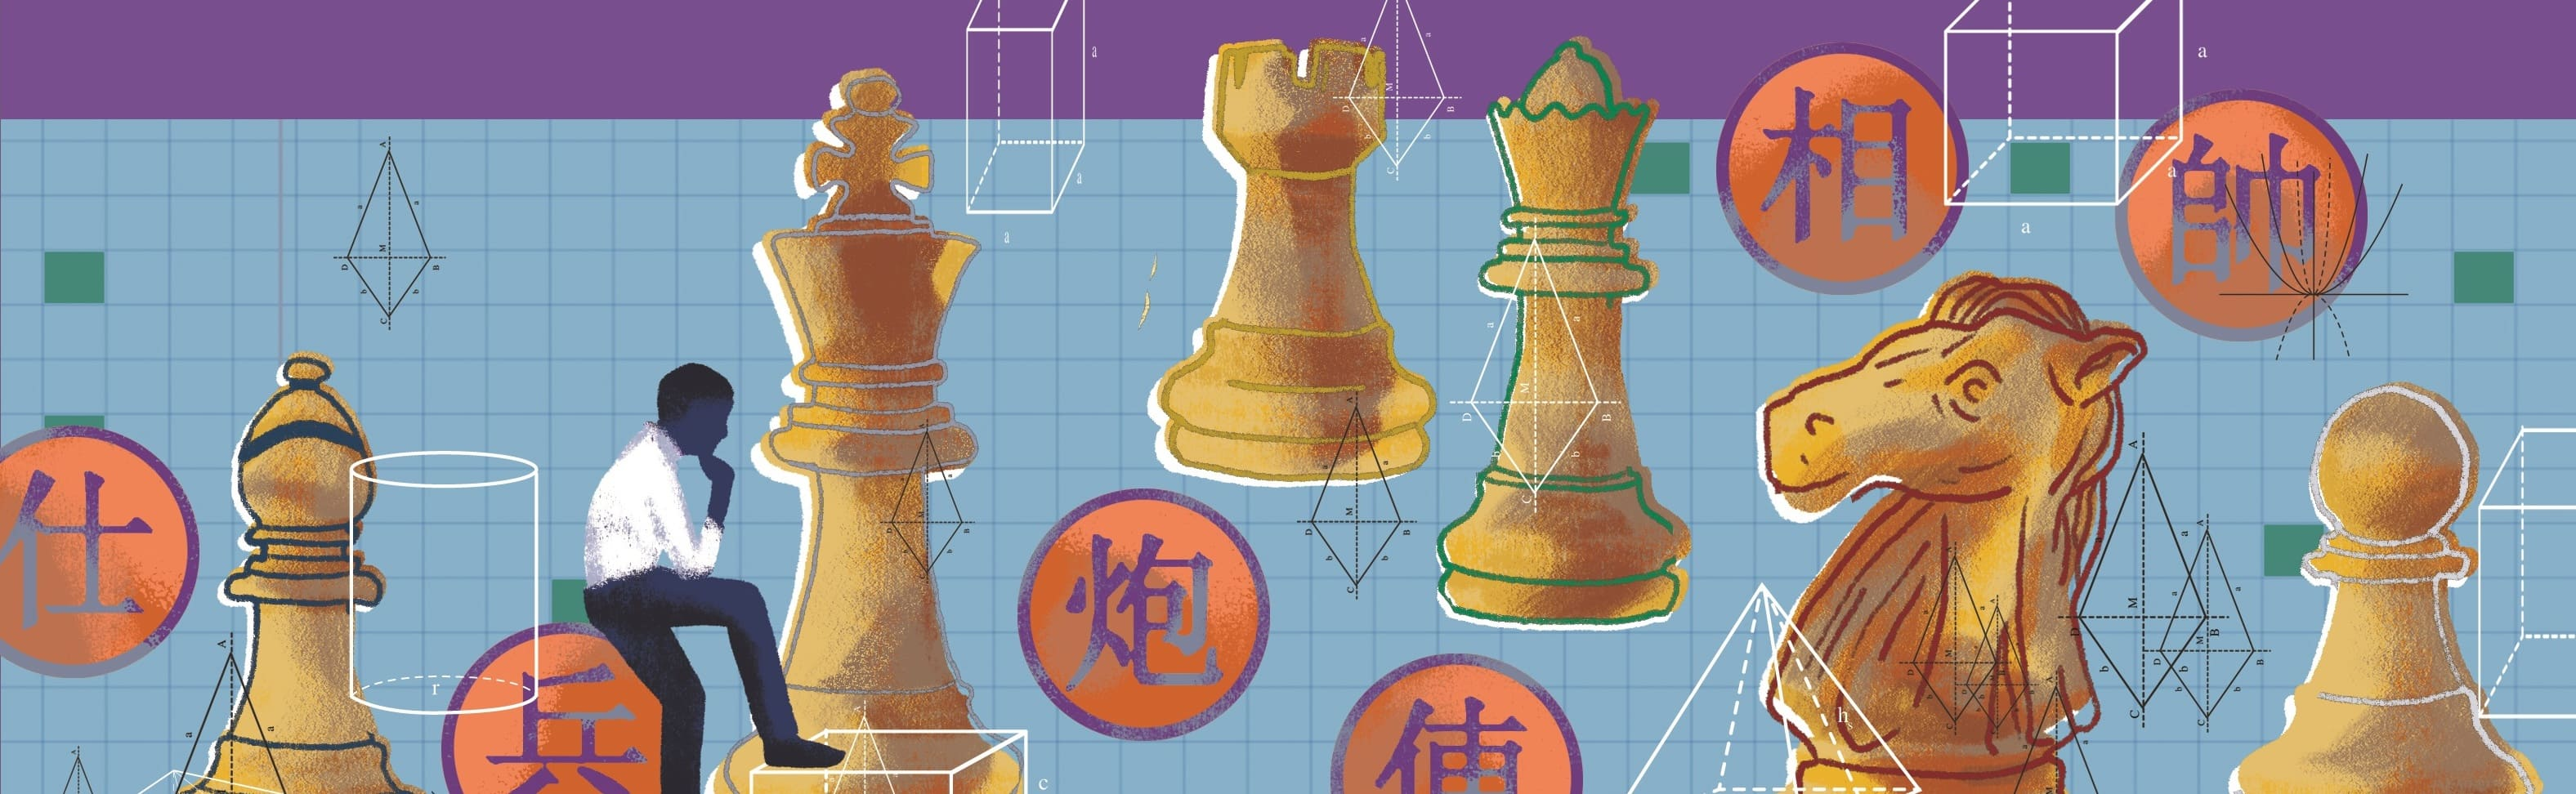
\includegraphics[width=19.3cm]{../bannergocco}}}
\AddToShipoutPicture*{\put(164,555){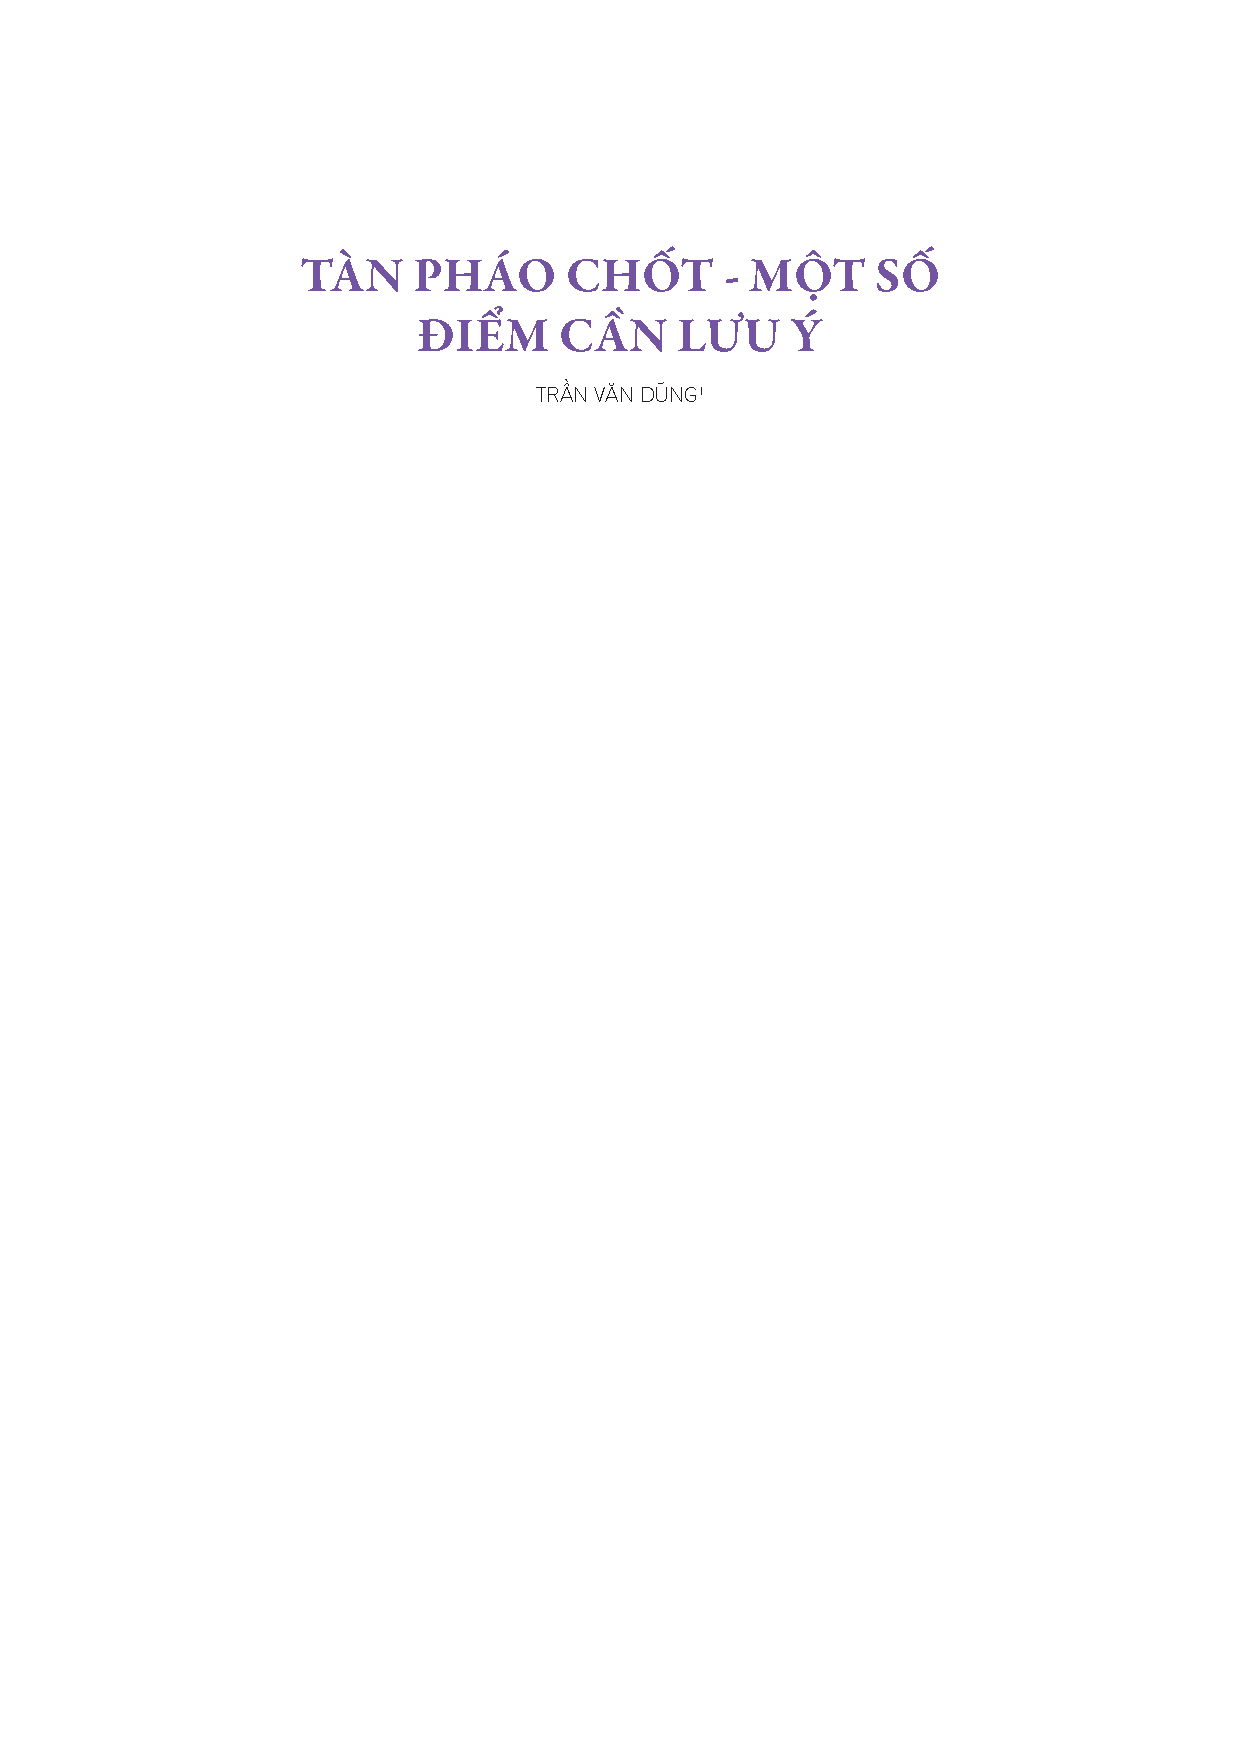
\includegraphics[scale=1]{../tieude2.pdf}}} 
\centering
\endgroup

\vspace*{150pt}

\begin{multicols}{2}
	\textit{Quân} và \textit{Thế} là $2$ yếu tố quan trọng không thể tách rời trong mỗi cuộc cờ. Khi nhắc đến \textit{Quân} là nhắc đến sức mạnh về vật chất: bên nào số lượng quân hơn, binh chủng đa dạng hơn thì hiển nhiên bên đó đang chiếm ưu thế. Trong khi đó, \textit{Thế} là một khái niệm chung chung, có vẻ khá mơ hồ, bao gồm nhiều yếu tố như: lộ quân thông thoáng, các quân lực trái -- phải, tiền -- hậu phối hợp hài hòa, đội hình ưu việt, nắm quyền chủ động… Như vậy, một cách đầy đủ và khái quát nhất, \textit{Thế} sẽ bao gồm cả vị trí lẫn mỗi liên quan của nó với các quân khác (kể cả quân đối phương). Chúng ta cùng nhau xét lần lượt các vấn đề then chốt:
	\vskip 0.1cm
	\textit{Về vị trí}: Trên bàn cờ luôn luôn tồn tại những vị trí tốt và vị trí xấu. Nếu có được vị trí tốt thì sức mạnh cũng như tính chiến đấu của các quân sẽ được phát huy hiệu quả; ngược lại, chỗ đứng chưa tốt thì những yếu tố đó sẽ bị hạn chế. Những quân chủ lực dù cơ động, linh hoạt nhưng đứng ở chỗ tối, trong góc hoặc đường biên thì chẳng thể gây nguy hiểm lên trận địa đối phương mà còn có thể trở thành điểm công kích cho đối thủ: Xe, Pháo nằm ở các lộ $4$, $5$, $6$ sẽ có tính uy hiếp cao;  Quân Mã nằm ở giữa bàn cờ rõ ràng linh hoạt hơn rất nhiều khi khống chế được 8 điểm. Do vậy, khởi đầu mỗi ván đấu, đôi bên cần nhanh chóng đưa các quân chủ lực đến vị trí xung yếu nhằm kiểm soát thế trận, hạn chế đưa quân vào những vị trí yếu đồng thời cũng tìm cách phong tỏa tối đa sức mạnh cũng như tầm hoạt động của quân đối phương.
	\vskip 0.1cm
	\textit{Về sự phối hợp các quân}: Là mối liên quan giữa các quân với nhau (Liệu chúng có liên kết phối hợp, hỗ trợ nhau để trở nên vững chắc hơn hơn, hay cản trở, hạn chế khả năng hoạt động của nhau ?). Sau giai đoạn khai cuộc và bước vào tiền trung cuộc là thời điểm đôi bên gần như đã bố trí xong đội hình, các quân cùng nhau phối hợp để trở thành một khối thống nhất, có mục tiêu chung. Sức mạnh của khối này có thể sẽ tăng hay giảm tùy theo diễn biến thực tế của mỗi ván đấu.
	\vskip 0.1cm
	\textit{Về mối liên quan với quân đối phương}: Là sự xung khắc, mâu thuẩn để nhằm hạn chế sức mạnh, tầm hoạt động của các quân giữa $2$ bên với nhau. Nếu mâu thuẫn lên đến đỉnh điểm, sẽ xảy ra các tình huống đổi quân, tiêu diệt lẫn nhau. Điều này cũng dẫn đến quy luật: các quân bên này phát huy càng cao sức mạnh của mình thì càng hạn chế sức mạnh của các quân phía đối thủ và ngược lại. Tất nhiên, trong trường hợp hai bên đều có những nước đi chính xác thì thế cờ sẽ dần đi vào trạng thái cân bằng. Chung quy lại, mối liên quan này thực chất là một cuộc đấu tranh quyết liệt để giành giật không gian bàn cờ, nhằm chiếm quyền chủ động, mục đích cuối cùng là lời quân, lời chất, để rồi giành lấy thắng lợi.
	Để hiểu hơn những vấn đề này, tác giả sẽ gửi tới bạn đọc của Pi vài ví dụ tiêu biểu nói về những điểm yếu thường gặp và cách khai thác để có thể áp dụng trong những ván đấu thực chiến:
	\begin{figure}[H]
		\vspace*{-5pt}
		\centering
		\captionsetup{labelformat= empty, justification=centering}
		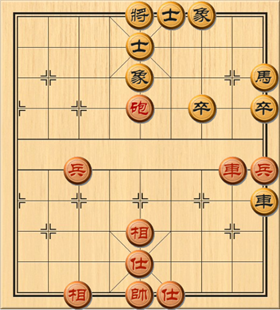
\includegraphics[width= 0.35\textwidth]{1}
		\caption{\small\textit{\color{gocco}Hình $1$.}}
		\vspace*{-10pt}
	\end{figure}
	$1.$ Hình $1$, Quân lực $2$ bên hoàn toàn tương đồng, cục diện có vẻ bình ổn. Tuy nhiên, khi xét kỹ thì sẽ thấy, bên Đen lộ ra một điểm yếu chết người đó là trục lộ $4$ (trục lộ $6$ của Đỏ). Đỏ được quyền đi trước và chớp lấy thời cơ như sau:
	\vskip 0.1cm
	$\pmb{1)}$	X$2-6$ X$9-2$\quad  $\pmb{2)}$ Tg$5-6$ X$2/6$ $(*)$\quad $\pmb{3)}$ C$7.1$ M$9/8$\quad $\pmb{4)}$ P$5/1$ M$8.7$ $(**)$\quad $\pmb{5)}$ X$6.2$ C$7.1$ \quad $\pmb{6)}$ C$7.1$ M$7.6$\quad $\pmb{7)}$ C$7.1$ M$6.5$\quad $\pmb{8)}$ X$4/3$ M$5.7$\quad $\pmb{9)}$ C$7.1$ M$7/6$\quad $\pmb{10)}$ X$4.3$ $(***)$ (Đỏ chiếm ưu lớn).
	\vskip 0.1cm
	\textit{$(*)$: Nhận thấy yếu điểm, Đỏ nhanh chóng bình Xe rồi bình Tướng nhằm tạo sát cục, buộc Đen phải đem xe về tuyến đáy phòng thủ.
	\vskip 0.1cm
	$(**)$: Đỏ tiếp tục đem chốt sang sông trợ chiến. Vì Xe không thể di chuyển nên lúc này phương án duy nhất Đen có thể chơi là điều Mã biên để đuổi Pháo của Đỏ.
	\vskip 0.1cm
	$(***)$: Những diễn biến vừa rồi, Đỏ liên tục đẩy Chốt tiến sát cửu cung của Đen. Mặc dù Đen cũng rất nỗ lực trong việc đưa Mã lên quấy rối nhưng Đỏ có những nước điều Xe hóa giải cùng đơn giản. Nước tiếp theo Đỏ có nước C$7.6$ dọa sát, dù cho Đen nhìn thấy nhưng cũng rất khó để chống đỡ, chiến thắng dành cho Đỏ chỉ còn là vấn đề về thời gian.}
	\begin{figure}[H]
		\vspace*{-5pt}
		\centering
		\captionsetup{labelformat= empty, justification=centering}
		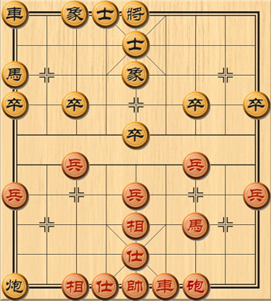
\includegraphics[width= 0.35\textwidth]{2}
		\caption{\small\textit{\color{gocco}Hình $2$.}}
		\vspace*{-10pt}
	\end{figure}
	$2.$ Hình $2$, quân lực và thể loại binh chủng của đôi bên là ngang nhau, Đen đang có Pháo cắm đáy ở phía trên nhưng chưa thể phối hợp, liên kết với Xe, Mã ở hậu phương. Tuy Đỏ chưa có quân nào xâm nhập phòng tuyến của địch nhưng đang có cơ hội phối hợp tác chiến, nhận thấy cánh trái của Đen đang hoàn toàn trống trải, Đỏ đi trước và ra đòn như sau:
	\vskip 0.1cm
	$\pmb{1)}$ P$3-2$ X$1-2$\quad  $\pmb{2)}$ P$2.9$ X$2.2$\quad $\pmb{3)}$ P$2-1$ T$5.3$\quad $\pmb{4)}$ X$4-2$ X$2-6$\quad $\pmb{5)}$ X$2.9$ S$5/6$ $(*)$\quad $\pmb{6)}$ M$3.2$ T$3/5$\quad $\pmb{7)}$ M$2.3$ X$6-7$\quad  $\pmb{8)}$ M$3/5$ $(**)$ S$4.5$\quad $\pmb{9)}$ Tg$5-4$ Tg$5-4$\quad $\pmb{10)}$ X$2-4$ Tg$4.1$\quad $\pmb{11)}$ X$4-7$ X$7/2$ $(***)$\quad $\pmb{12)}$ X$7/2$ X$7-9$\quad $\pmb{13)}$ X$7-9$ $(****)$ $(1-0)$
	\vskip 0.1cm
	\textit{$(*)$: Nhận thấy tuyến đáy của Đen là điểm có thể công kích, Đỏ ngay lập tức điều Pháo và Xe uy hiếp, sẵn sàng chờ cơ hội để chiếu rút. Ở chiều hướng ngược lại, Đen cũng nhanh chóng đưa Xe ra nhằm chiếm lấy trục lộ quan trọng.
	\vskip 0.1cm
	$(**)$: Chỉ với Xe và Pháo chưa thể tạo ra sát cục, Đỏ tiếp tục đem Mã lên dồn lực tấn công. Bộ ba Xe Pháo Mã của Đen nằm tản mác, không thế liên kết phòng thủ, Đen ở ``tình thế ngàn cân treo sợi tóc".
	\vskip 0.1cm
	$(***)$: Đỏ tiếp tục đem Tướng ra hỗ trợ dọa sát, giúp chiến Xe thoải mái càn quét tuyến đáy của Đen, đặt nền tảng cho chiến thắng.
	\vskip 0.1cm
	$(****)$: Đen cố gắng thoái Xe mời đổi nhằm giảm bớt áp lực nhưng vẫn không thể thay đổi được cục diện. Sau khi ăn Mã, Đỏ chuẩn bị có những đòn phối hợp Xe Mã tạo sát, Đen rất khó chống đỡ.}
	\begin{figure}[H]
		\vspace*{-5pt}
		\centering
		\captionsetup{labelformat= empty, justification=centering}
		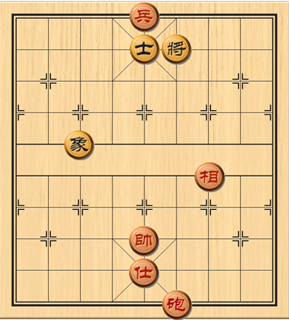
\includegraphics[width= 0.35\textwidth]{3}
		\caption{\small\textit{\color{gocco}Hình $3$.}}
		\vspace*{-10pt}
	\end{figure}
	$3.$ Hình $3$, quân lực đôi bên khá đồng đều, Xe Đỏ đang bị phong tỏa, chốt đầu của Đen đang được giữ chặt. Điểm yếu duy nhất của Đen là Mã nhập cung, nếu tiếp theo Đen có thể tung Mã lên tham chiến thì chắc chắn Đỏ sẽ khó lòng chống đỡ. Tuy nhiên, Đỏ được quyền đi trước và có những nước đi bất ngờ xoay chuyển tình thế:
	\vskip 0.1cm
	$\pmb{1)}$	X$2.1$ X$8.5$\quad  $\pmb{2)}$ P$5.4$ T$7.5$ $(*)$\quad $\pmb{3)}$ M$8.6$ X$8/6$ $(**)$\quad $\pmb{4)}$ P$7-3$ X$8-7$\quad $\pmb{5)}$ M$6.8$ $(***)$ P$3-4$\quad $\pmb{6)}$ M$8.6$ $(1-0)$
	\vskip 0.1cm
	\textit{$(*)$: Nhận thấy điểm yếu Mã nhập cung của Đen, Đỏ tung đòn phế Xe một cách dứt khoát và uy lực. Đen buộc phải dùng Xe bắt lại Xe Đỏ và hệ quả là Chốt đầu không còn quân bảo vệ, Đỏ liền tấn Pháo chiếu Tướng uy hiếp. Lúc này Đen không thể di chuyển Mã vì Đỏ sẽ đi P$7-5$ sát cục Pháo trùng ngay lập tức.
	\vskip 0.1cm
	$(**)$: Đỏ tiếp tục đưa Mã xâm nhập, gây áp lực lớn lên trận địa đối phương, Đen buộc phải đưa xe về phòng thủ một cách bị động.
	\vskip 0.1cm
	$(***)$: Đỏ lần lượt điều Pháo rồi lại tung Mã liên tục uy hiếp, dọa chiếu bí. Điểm yếu Mã nhập cung với Pháo đầu đóng chặt là quá lớn, Đen mặc dù nhìn thấy trước nhưng vô phương chống đỡ. Đỏ giành chiến thắng.}
	\vskip 0.1cm
	\textit{Chú thích}: C: Chốt, X: Xe, M: Mã, P: Pháo, Tg: Tướng, S: Sĩ, T: Tượng. 
	\vskip 0.1cm
	\textbf{\color{gocco}Câu đố kỳ này:} Đỏ được quyền đi trước, làm thể nào để khai thác những điểm yếu của đối phương để giành lấy ưu thế?
	\begin{figure}[H]
		\vspace*{-5pt}
		\centering
		\captionsetup{labelformat= empty, justification=centering}
		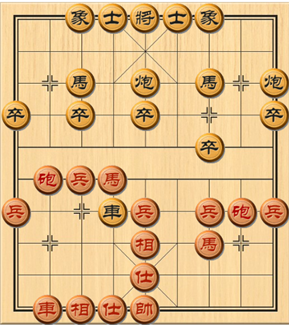
\includegraphics[width= 0.35\textwidth]{4}
		\caption{\small\textit{\color{gocco}Hình $4$.}}
		\vspace*{-10pt}
	\end{figure}
	\textit{Đáp án tham khảo}: $\pmb{1)}$ C$3.1$ X$4.2$\quad  $\pmb{2)}$ X$8.3$ P$5-6$\quad  $\pmb{3)}$ P$2-4$ M$7.6$\quad $\pmb{4)}$ P$4.4$ M$6.4$\quad $\pmb{5)}$ P$4/6$ (Đen mất xe, Đỏ chiếm ưu thế lớn).
	\begin{figure}[H]
		\vspace*{-5pt}
		\centering
		\captionsetup{labelformat= empty, justification=centering}
		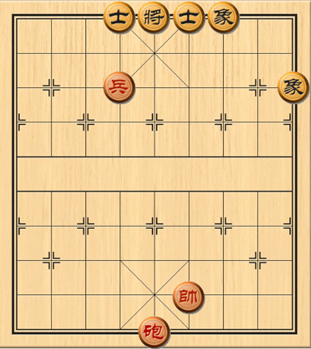
\includegraphics[width= 0.35\textwidth]{5}
		\caption{\small\textit{\color{gocco}Hình $5$.}}
		\vspace*{-10pt}
	\end{figure}
	\textit{Đáp án tham khảo}: $\pmb{1)}$ X$1-4$ S$4.5$\quad  $\pmb{2)}$ X$4.4$ M$4.3$\quad $\pmb{3)}$ X$9.2$ M$3.2$\quad $\pmb{4)}$ X$9-8$ X$1-2$\quad $\pmb{5)}$ X$8.7$ M$3/2$\quad $\pmb{6)}$ C$7.1$ Ms$.1$\quad $\pmb{7)}$ X$4-7$ C$3.1$\quad  $\pmb{8)}$ X$7/3$ C$1.1$\quad $\pmb{9)}$ X$7-8$ (Đen chết Mã, Đỏ ưu thế lớn).	
\end{multicols}




